\chapter{Probabilités}

\minitoc

\section{Rappels et compléments sur les ensembles}

\subsection{Ensembles finis}

\begin{defi}
Un ensemble \(E\) est dit fini s'il contient un nombre fini d'éléments.

Le nombre d'éléments de \(E\) est appelé cardinal de \(E\) et est noté \(\abs{E}\), \(\Card E\) ou encore \(\#E\).
\end{defi}

\begin{theo}
Soient \(E\) un ensemble fini et \(A\subset E\) une partie de \(E\).

Alors \(A\) est un ensemble fini.

De plus, on a : \[\Card A\leq\Card E\] avec égalité si, et seulement si, \(A=E\).
\end{theo}

\begin{theo}
Soient \(E\) et \(F\) deux ensembles finis de même cardinal et une fonction \(f:E\to F\).

Les trois propositions suivantes sont équivalentes :

\begin{enumerate}
    \item \(f\) est une bijection \\
    \item \(f\) est une injection \\
    \item \(f\) est une surjection.
\end{enumerate}
\end{theo}

\subsection{Dénombrement des ensembles finis}

Soient \(E\) un ensemble fini et \(A,B\in\P{E}\).

On a :

\begin{description}
    \item[] \(\Card A\union B=\Card A+\Card B\) si \(A\) et \(B\) sont disjoints \\
    \item[] \(\Card A\union B=\Card A+\Card B-\Card A\inter B\) \\
    \item[] \(\Card E\excluant A=\Card E-\Card A\) \\
    \item[] \(\Card A\times B=\Card A\times\Card B\) \\
    \item[] \(\Card B^A=\Card\F{A}{B}=\paren{\Card B}^{\Card A}\) \\
    \item[] \(\Card\P{E}=2^{\Card E}\) \\
    \item[] \(\Card E^p=\paren{\Card E}^p\).
\end{description}

Soit \(p\in\interventierii{0}{n}\).

On appelle :

\begin{description}
    \item[] \(p\)-arrangement de \(E\) tout \(p\)-uplet d'éléments de \(E\) deux à deux distincts ; \\
    \item[] \(p\)-combinaison de \(E\) toute partie de \(E\) contenant \(p\) éléments.
\end{description}

On a alors, en notant \(n\) le cardinal de \(E\) :

\begin{description}
    \item[] le nombre de \(p\)-arrangements de \(E\) est \(\arr{p}{n}=\dfrac{n!}{\paren{n-p}!}\) \\
    \item[] le nombre de \(p\)-combinaisons de \(E\) est \(\comb{p}{n}=\binom{p}{n}=\dfrac{n!}{p!\,\paren{n-p}!}\)
\end{description}

Enfin, \(\arr{p}{n}\) est aussi le nombre d'injections d'un ensemble de cardinal \(p\) vers \(E\). En particulier, si \(p=n\) et en notant \(\S{E}\) l'ensemble des bijections de \(E\) vers \(E\) : \[\Card\S{E}=n!\]

\begin{exoex}
Soient \(k,n\in\Ns\) tels que \(k\leq n\).

Une urne contient \(n\) boules numérotées de \(1\) à \(n\). On tire \(k\) boules dans cette urne.

Donner le nombre de résultats possibles en fonction du type de tirage :

\begin{enumerate}
    \item On tire \(k\) boules simultanément. \\
    \item On tire \(k\) boules une par une, avec remise. \\
    \item On tire \(k\) boules une par une, sans remise.
\end{enumerate}
\end{exoex}

\begin{corr}~\\
\begin{enumerate}
    \item Il y a \(\binom{k}{n}\) résultats possibles. \\
    \item Il y a \(n^k\) résultats possibles. \\
    \item Il y a \(\arr{k}{n}\) résultats possibles.
\end{enumerate}
\end{corr}

\begin{exoex}[Mines-Télécom 2016]
Soit \(E\) un ensemble fini dont on note \(n\) le cardinal.

Donner le cardinal des ensembles suivants :

\begin{enumerate}
    \item \(E_1=\accol{\paren{X,Y}\in\P{E}^2\tq\accol{X;Y}\text{ est une partition de }E}\) ; \\
    \item \(E_2=\accol{\paren{X,Y}\in\P{E}^2\tq X\inter Y=\ensvide}\) ; \\
    \item \(E_3=\accol{\paren{X,Y}\in\P{E}^2\tq X\union Y=E}\) ; \\
    \item \(E_4=\accol{\paren{X,Y}\in\P{E}^2\tq X\subset Y}\) ; \\
    \item \(E_5=\accol{\paren{X,Y,Z}\in\P{E}^3\tq X\union Y\union Z=E}\).
\end{enumerate}
\end{exoex}

\begin{corr}
On a :

\begin{enumerate}
    \item \(\Card E_1=2^n-2\) \\
    \item \(\Card E_2=\sum_{k=0}^{n}\binom{k}{n}2^{n-k}=3^n\) \\
    \item \(\Card E_3=3^n\) \\
    \item \(\Card E_4=3^n\) \\
    \item \(\Card E_5=7^n\)
\end{enumerate}
\end{corr}

\section{Espaces probabilisés}

\subsection{Cadre formel}

\subsubsection{Univers}

On considère un ensemble fini non-vide \(\Omega\) appelé l'univers.

\begin{ex}
\begin{itemize}
    \item On lance un dé une fois : \(\Omega=\interventierii{1}{6}\). \\
    \item On lance un dé deux fois : \(\Omega=\interventierii{1}{6}^2\). \\
    \item On lance un dé \(n\) fois : \(\Omega=\interventierii{1}{6}^n\).
\end{itemize}
\end{ex}

\begin{rem}
En pratique, on ne précisera pas quel est l'univers (il y a beaucoup de façons de modéliser une situation et la modélisation choisie ne change pas les probabilités obtenues).
\end{rem}

\subsubsection{Événements}

Les parties de \(\Omega\) sont appelées les événements.

\begin{ex}
\begin{itemize}
    \item Expérience aléatoire : on lance un dé une fois. \\ Univers : \(\Omega=\interventierii{1}{6}\). \\ Événement \guillemets{le résultat vaut \(6\)} : \(\accol{6}\). \\ Événement \guillemets{le résultat est pair} : \(\accol{2;4;6}\). \\
    \item Expérience aléatoire : on lance un dé deux fois. \\ Univers : \(\Omega=\interventierii{1}{6}^2\). \\ Événement \guillemets{les deux lancers donnent le même résultat} : \(\accol{\paren{1,1};\paren{2,2};\paren{3,3};\paren{4,4};\paren{5,5};\paren{6,6}}\).
\end{itemize}
\end{ex}

\begin{defi}
L'ensemble vide \(\ensvide\) est un événement, appelé l'événement impossible.

L'événement \(\Omega\) est appelé l'événement certain.

Les événements qui ne contiennent qu'un seul élément (\ie les singletons) sont appelés événements élémentaires.
\end{defi}

\begin{defi}
Deux événements sont dits incompatibles (ou disjoints) si leur intersection est vide.
\end{defi}

\begin{defi}[Système complet d'événements]
Soient \(\Omega\) un univers et \(N\in\Ns\).

On appelle système complet d'événements toute famille \(\paren{A_1,\dots,A_N}\in\P{\Omega}^N\) d'événements deux à deux incompatibles telle que \[\bigunion_{n=1}^NA_n=\Omega.\]
\end{defi}

\subsubsection{Probabilité}

\begin{defi}[Probabilité]
Soit \(\Omega\) un univers.

On appelle probabilité sur \(\Omega\) toute application \(\prem:\P{\Omega}\to\intervii{0}{1}\) telle que :

\begin{enumerate}
    \item \(\proba{\Omega}=1\) \\
    \item Pour tout entier \(N\in\Ns\) et toute famille \(\paren{A_1,\dots,A_N}\in\P{\Omega}^N\) d'événements deux à deux incompatibles : \[\proba{\bigunion_{n=1}^NA_n}=\sum_{n=1}^N\proba{A_n}.\]
\end{enumerate}
\end{defi}

\begin{defi}[Espace probabilisé]
Un couple \(\groupe{\Omega}[\prem]\), où \(\Omega\) est un univers et \(\prem\) est une probabilité sur \(\Omega\), est appelé un espace probabilisé.
\end{defi}

\begin{rem}
Soit \(\groupe{\Omega}[\prem]\) un espace probabilisé.

On a : \[\proba{\ensvide}=0.\]
\end{rem}

\begin{dem}
On a \(\ensvide=\ensvide\union\ensvide\) (événements incompatibles) donc \(\proba{\ensvide}=\proba{\ensvide}+\proba{\ensvide}\).

Donc \(\proba{\ensvide}=0\).
\end{dem}

\begin{rem}
Soit \(\Omega\) un univers.

Dans ce chapitre, on note généralement \(\conj{A}\) le complémentaire dans \(\Omega\) de l'événement \(A\in\P{\Omega}\).

Le complémentaire d'une partie n'est jamais noté ainsi dans le cadre de la topologie (notation alors réservée à l'adhérence).
\end{rem}

\begin{prop}
Soient \(\groupe{\Omega}[\prem]\) un espace probabilisé et \(A,B\in\P{\Omega}\) deux événements.

\begin{enumerate}
    \item Si \(A\subset B\) alors \(\proba{B\excluant A}=\proba{B}-\proba{A}\). En particulier, on a \(\proba{A}\leq\proba{B}\). \\
    \item On a \(\proba{\conj{A}}=1-\proba{A}\). \\
    \item On a \(\proba{A\union B}=\proba{A}+\proba{B}-\proba{A\inter B}\).
\end{enumerate}
\end{prop}

\begin{dem}[1]
On a \(B=A\union\paren{B\excluant A}\) (réunion disjointe) donc \(\proba{B}=\proba{A}+\proba{B\excluant A}\).
\end{dem}

\begin{dem}[2]
Découle du (1) en prenant \(B=\Omega\).
\end{dem}

\begin{dem}[3]
On a \(A\union B=\paren{A\excluant B}\union\paren{A\inter B}\union\paren{B\excluant A}\) (réunion disjointe).

Donc \(\proba{A\union B}=\proba{A\excluant B}+\proba{A\inter B}+\proba{B\excluant A}\).

D'autre part, on a \(\begin{dcases}
A=\paren{A\excluant B}\union\paren{A\inter B} \\
B=\paren{B\excluant A}\union\paren{A\inter B}
\end{dcases}\) (réunions disjointes).

Donc on a \(\begin{dcases}
\proba{A}=\proba{A\excluant B}+\proba{A\inter B} \\
\proba{B}=\proba{B\excluant A}+\proba{A\inter B}
\end{dcases}\)

D'où la formule.
\end{dem}

\begin{prop}[Sous-additivité]
Soient \(\groupe{\Omega}[\prem]\) un espace probabilisé et \(N\in\Ns\).

Pour toute famille d'événements \(\paren{A_1,\dots,A_N}\in\P{\Omega}^N\), on a : \[\proba{\bigunion_{n=1}^NA_n}\leq\sum_{n=1}^N\proba{A_n}.\]
\end{prop}

\begin{dem}
On pose \(\quantifs{\forall k\in\interventierii{1}{N}}A_k\prim=A_k\excluant\bigunion_{i=1}^{k-1}A_i\) de sorte que \(\bigunion_{k=1}^NA_k=\bigunion_{k=1}^NA_k\prim\) (réunion disjointe).

On a alors : \[\begin{WithArrows}
\proba{\bigunion_{k=1}^NA_k}&=\sum_{k=1}^N\proba{A_k\prim} \Arrow{car \(\quantifs{\forall k\in\interventierii{1}{N}}A_k\prim\subset A_k\)} \\
&\leq\sum_{k=1}^N\proba{A_k}
\end{WithArrows}\]
\end{dem}

\subsubsection{Distribution de probabilités}

\begin{defi}
Soit \(\Omega\) un univers.

On appelle distribution de probabilités sur \(\Omega\) toute famille \(\paren{p_\omega}_{\omega\in\Omega}\) de réels positifs de somme \(1\) : \[\quantifs{\forall\omega\in\Omega}p_\omega\geq0\qquad\text{et}\qquad\sum_{\omega\in\Omega}p_\omega=1.\]
\end{defi}

\begin{prop}
Soit \(\Omega\) un univers.

La donnée d'une probabilité sur \(\Omega\) revient à la donnée d'une distribution de probabilités sur \(\Omega\).
\end{prop}

\begin{dem}
\analyse

Soient \(\prem\) une probabilité sur \(\Omega\) et \(A\subset\Omega\).

On a \(A=\bigunion_{\omega\in A}\accol{\omega}\) (réunion disjointe).

Donc, en posant \(\quantifs{\forall\omega\in\Omega}p_\omega=\proba{\accol{\omega}}\), on a : \[\proba{A}=\sum_{\omega\in A}\proba{\accol{\omega}}=p_\omega.\]

On a bien \(\begin{dcases}
\quantifs{\forall\omega\in\Omega}p_\omega\geq0 \\
\sum_{\omega\in\Omega}p_\omega=\proba{\Omega}=1
\end{dcases}\)

Donc \(\paren{p_\omega}_{\omega\in\Omega}\) est une distribution de probabilités sur \(\Omega\).

\synthese

Soit \(\paren{p_\omega}_{\omega\in\Omega}\) une distribution de probabilités sur \(\Omega\).

On pose : \[\fonction{\prem}{\P{\Omega}}{\R}{A}{\sum_{\omega\in A}p_\omega}\]

Montrons que \(\prem\) est une probabilité sur \(\Omega\).

Soient \(N\in\Ns\) et \(A_1,\dots,A_N\in\P{\Omega}\) des événements deux à deux incompatibles.

On a : \[\begin{WithArrows}
\proba{\bigunion_{i=1}^NA_i}&=\sum_{\omega\in\bigunion_{i=1}^NA_i}p_\omega \Arrow{car \(\bigunion_{i=1}^NA_i\) est une réunion disjointe} \\
&=\sum_{i=1}^N\sum_{\omega\in A_i}p_\omega \\
&=\sum_{i=1}^N\proba{A_i}.
\end{WithArrows}\]

De plus, on a \(\proba{\Omega}=\sum_{\omega\in\Omega}p_\omega=1\).

Donc \(\prem\) est une probabilité sur \(\Omega\).
\end{dem}

\subsection{Exemple : probabilité uniforme sur un ensemble fini}

\begin{defi}[Probabilité uniforme]
Soit \(\Omega\) un univers.

On appelle probabilité uniforme sur \(\Omega\) la probabilité \(\prem\) définie par : \[\quantifs{\forall A\in\P{\Omega}}\proba{A}=\dfrac{\Card A}{\Card\Omega}.\]

Pour cette probabilité, tous les événements élémentaires sont équiprobables, de probabilité \(\dfrac{1}{\Card\Omega}\).
\end{defi}

\begin{ex}[Lancer d'un dé]
On lance un dé (non-pipé, à six faces).

Le résultat peut être modélisé par l'univers \(\Omega=\interventierii{1}{6}\) muni de la probabilité uniforme.
\end{ex}

\begin{exoex}
On tire simultanément trois cartes dans un jeu de trente-deux cartes. On suppose que tous les tirages sont équiprobables.

\begin{enumerate}
    \item Quelle est la probabilité de tirer trois as ? \\
    \item Quelle est la probabilité de tirer trois cartes qui se suivent ? \\
    \item Quelle est la probabilité de tirer deux rois et une dame ?
\end{enumerate}
\end{exoex}

\begin{corr}[1]~\\
On a \(\Card\Omega=\binom{3}{32}\).

On note \(A\) l'événement \guillemets{on tire trois as}.

On a \(\Card A=\binom{3}{4}\).

Donc : \[\begin{aligned}
\proba{A}&=\dfrac{\Card A}{\Card\Omega} \\
&=\dfrac{\binom{3}{4}}{\binom{3}{32}} \\
&=\dfrac{\frac{4\times3\times2}{3\times2\times1}}{\frac{32\times31\times30}{3\times2\times1}} \\
&=\dfrac{4\times3\times2}{32\times31\times30} \\
&=\dfrac{1}{4\times31\times10} \\
&=\dfrac{1}{1240}.
\end{aligned}\]
\end{corr}

\begin{corr}[2]
On note \(B\) l'événement \guillemets{on tire trois cartes qui se suivent}.

On a \(\Card B=6\times4^3\).

Donc : \[\begin{aligned}
\proba{B}&=\dfrac{6\times4^3}{\frac{32\times31\times30}{3\times2\times1}} \\
&=\dfrac{2\times3\times6\times2^6}{30\times31\times32} \\
&=\dfrac{2^2\times3}{5\times31} \\
&=\dfrac{12}{155}.
\end{aligned}\]
\end{corr}

\begin{corr}[3]
On note \(C\) l'événement \guillemets{on tire deux rois et une dame}.

On a \(\Card C=\binom{2}{4}\times\binom{1}{4}=4\times6\).

Donc : \[\begin{aligned}
\proba{C}&=\dfrac{6\times4}{\frac{32\times31\times30}{3\times2\times1}} \\
&=\dfrac{2^4\times3^2}{2^5\times31\times2\times5\times3} \\
&=\dfrac{3}{2^2\times5\times31} \\
&=\dfrac{3}{620}.
\end{aligned}\]
\end{corr}

\section{Conditionnement}

\subsection{Définitions}

On considère un espace probabilisé \(\groupe{\Omega}[\prem]\).

\begin{defi}
Soient \(A,B\in\P{\Omega}\) deux événements tels que \(\proba{B}\not=0\).

On appelle probabilité conditionnelle de \(A\) sachant \(B\) le réel : \[\probacond{A}{B}=\proba{A\mid B}=\dfrac{\proba{A\inter B}}{\proba{B}}.\]
\end{defi}

\begin{rem}\thlabel{rem:probaIntersectionDeuxÉvénements}
On a donc \(\proba{A\inter B}=\proba{B}\proba{A\mid B}\).
\end{rem}

\begin{exoex}
On lance deux dés.

\begin{enumerate}
    \item Quelle est la probabilité d'avoir au total au moins \(10\) ? \\
    \item Quelle est la probabilité d'avoir au total au moins \(10\) sachant que l'un des deux dés donne \(2\) ? \\
    \item Quelle est la probabilité d'avoir au total au moins \(10\) sachant que l'un des deux dés donne \(6\) ?
\end{enumerate}
\end{exoex}

\begin{corr}[1]
On a l'univers \(\Omega=\interventierii{1}{6}^2\) de cardinal \(36\).

On note \(A\) l'événement \guillemets{avoir au total au moins 10}.

On a \(A=\accol{\paren{4,6};\paren{5,5};\paren{5,6};\paren{6,4};\paren{6,5};\paren{6,6}}\) donc \(\Card A=6\).

Donc \(\proba{A}=\dfrac{6}{36}=\dfrac{1}{6}\).
\end{corr}

\begin{corr}[2]
La probabilité est nulle.
\end{corr}

\begin{corr}[3]
On note \(A\) l'événement \guillemets{avoir au total au moins 10} et \(B\) l'événement \guillemets{l'un des deux dés donne 6}.

On a : \[\proba{A\mid B}=\dfrac{\proba{A\inter B}}{\proba{B}}=\dfrac{5}{11}.\]
\end{corr}

\begin{prop}
Soit \(B\) un événement de probabilité non-nulle.

L'application \(\prem_B:\P{\Omega}\to\intervii{0}{1}\) est une probabilité sur \(\Omega\).
\end{prop}

\subsection{Propriétés}

\subsubsection{Formule des probabilités composées}

\begin{prop}
Soient \(N\in\Ns\) et \(A_1,\dots,A_N\) des événements tels que \(\proba{A_1\inter\dots\inter A_{N-1}}\not=0\).

Alors \[\proba{A_1\inter\dots\inter A_N}=\proba{A_1}\probacond{A_2}{A_1}\probacond{A_3}{A_1\inter A_2}\dots\probacond{A_N}{A_1\inter\dots\inter A_{N-1}}.\]
\end{prop}

\begin{dem}
Découle de la \thref{rem:probaIntersectionDeuxÉvénements}, par récurrence sur \(N\).
\end{dem}

\subsubsection{Formule des probabilités totales}

\begin{prop}[Formule des probabilités totales]
Soient \(N\in\Ns\), \(\paren{A_1,\dots,A_N}\) un système complet fini d'événements et \(B\) un événement.

On a : \[\proba{B}=\sum_{n=1}^N\proba{B\inter A_n}=\sum_{n=1}^N\proba{B\mid A_n}\proba{A_n},\] avec la convention \(\proba{B\mid A_n}\proba{A_n}=0\) si \(\proba{A_n}=0\).
\end{prop}

\begin{dem}~\\
On a \(B=\bigunion_{n=1}^N\paren{A_n\inter B}\) (réunion disjointe).

Donc \[\begin{WithArrows}
\proba{B}&=\sum_{n=1}^N\proba{A_n\inter B} \Arrow[tikz={text width=4cm}]{selon la formule des probabilités composées} \\
&=\sum_{n=1}^N\proba{A_n}\proba{B\mid A_n}.
\end{WithArrows}\]
\end{dem}

\subsubsection{Formules de Bayes}

\begin{prop}[Formule de Bayes]
\begin{itemize}
    \item Soient \(A\) et \(B\) deux événements de probabilité non-nulle. On a : \[\proba{A\mid B}=\dfrac{\proba{A}\proba{B\mid A}}{\proba{B}}=\dfrac{\proba{A}\proba{B\mid A}}{\proba{A}\proba{B\mid A}+\proba{\conj{A}}\proba{B\mid\conj{A}}}.\]
    \item Soient \(N\in\Ns\), \(\paren{A_1,\dots,A_n}\) un système complet fini d'événements de probabilité non-nulle, \(B\) un événement de probabilité non-nulle et \(k\in\interventierii{1}{N}\). On a : \[\proba{A_k\mid B}=\dfrac{\proba{A_k}\proba{B\mid A_k}}{\ds\sum_{n=1}^{N}\proba{A_n}\proba{B\mid A_n}}.\]
\end{itemize}
\end{prop}

\begin{exoex}
Dans une population de 60 millions d'individus, 6000 personnes sont porteuses d'un virus.

Il existe un test, mais celui-ci n'est pas complètement fiable :

Si un patient sain est testé, le résultat est négatif avec une probabilité de 98\%.

Si un patient malade est testé, le résultat est positif avec une probabilité de 99\%.

Un patient a fait un test dont le résultat est positif.

Quelle est la probabilité qu'il soit malade ?
\end{exoex}

\begin{corr}
On note \(M\) l'événement \guillemets{le patient est malade} et \(P\) l'événement \guillemets{le test est positif}.

On a : \[\begin{WithArrows}
\proba{M\mid P}&=\dfrac{\proba{M}\proba{P\mid M}}{\proba{M}\proba{P\mid M}+\proba{\conj{M}}\proba{P\mid\conj{M}}} \\
&=\dfrac{\num{e-4}\times\num{0.99}}{\num{e-2}\times\num{0.99}+\paren{1-\num{e-4}}\times\num{0.02}} \Arrow{on calcule} \\
&=\dfrac{1}{203}.
\end{WithArrows}\]
\end{corr}

\begin{exoex}
Je possède 20 dés : 18 sont non-pipés (probabilité uniforme sur \(\interventierii{1}{6}\)) et 2 sont pipés (une chance sur deux d'obtenir 6 quand on les lance).

Je prends l'un des 20 dés, le lance et obtiens 6.

Quelle est la probabilité que ce dé soit truqué ? Et si j'obtiens autre chose que 6 ?
\end{exoex}

\begin{corr}
On note \(P\) l'événement \guillemets{le dé est pipé} et \(S\) l'événement \guillemets{on obtient un 6}.

On a : \[\begin{WithArrows}
\proba{P\mid S}&=\dfrac{\proba{P}\proba{S\mid P}}{\proba{P}\proba{S\mid P}+\proba{\conj{P}}\proba{S\mid\conj{P}}} \\
&=\dfrac{\frac{1}{10}\times\frac{1}{2}}{\frac{1}{10}\times\frac{1}{2}+\frac{9}{10}\times\frac{1}{6}} \Arrow{on calcule} \\
&=\dfrac{1}{4}.
\end{WithArrows}\] et \[\begin{WithArrows}
\proba{P\mid\conj{S}}&=\dfrac{\proba{P}\proba{\conj{S}\mid P}}{\proba{P}\proba{\conj{S}\mid P}+\proba{\conj{P}}\proba{\conj{S}\mid\conj{P}}} \\
&=\dfrac{\frac{1}{10}\times\frac{1}{2}}{\frac{1}{10}\times\frac{1}{2}+\frac{9}{10}\times\frac{5}{6}} \Arrow{on calcule} \\
&=\dfrac{1}{16}.
\end{WithArrows}\]
\end{corr}

\section{Événements indépendants}

On considère toujours un espace probabilisé \(\groupe{\Omega}[\prem]\).

\begin{defi}
Deux événements \(A\) et \(B\) sont dits indépendants si on a : \[\proba{A\inter B}=\proba{A}\proba{B}.\]
\end{defi}

\begin{ex}
On pioche une carte dans un jeu de 52 cartes.

Les événements \guillemets{la carte est un 7} et \guillemets{la carte est un cœur} sont indépendants.
\end{ex}

\begin{rem}
Soient deux événements \(A\) et \(B\) tels que \(\proba{B}\not=0\).

Alors \[A\text{ et }B\text{ sont indépendants}\ssi\proba{A}=\proba{A\mid B}.\]
\end{rem}

\begin{dem}
On a : \[\begin{WithArrows}
A\text{ et }B\text{ sont indépendants}&\ssi\proba{A\inter B}=\proba{A}\proba{B} \Arrow{car \(\proba{B}\not=0\)} \\
&\ssi\dfrac{\proba{A\inter B}}{\proba{B}}=\proba{A} \\
&\ssi\proba{A\mid B}=\proba{A}.
\end{WithArrows}\]
\end{dem}

\begin{defi}
Soit \(N\in\Ns\).

Des événements \(A_1,\dots,A_N\) sont dits :

\begin{itemize}
    \item deux à deux indépendants si pour tous \(i,j\in\interventierii{1}{N}\) tels que \(i\not=j\) on a : \[\proba{A_i\inter A_j}=\proba{A_i}\proba{A_j}.\]
    \item mutuellement indépendants si pour tout \(J\subset\interventierii{1}{N}\) on a : \[\proba{\biginter_{j\in J}A_j}=\prod_{j\in J}\proba{A_j}.\]
\end{itemize}
\end{defi}

\begin{rem}
On a : \[\text{indépendance mutuelle}\imp\text{indépendance deux à deux}.\]

La réciproque est fausse.
\end{rem}

\begin{exoex}
Soient \(A\) et \(B\) deux événements indépendants.

Montrer que \(A\) et \(\conj{B}\) sont indépendants, que \(\conj{A}\) et \(B\) sont indépendants et que \(\conj{A}\) et \(\conj{B}\) sont indépendants.
\end{exoex}

\begin{corr}
On a \(\proba{A\inter B}=\proba{A}\proba{B}\).

Donc, comme \(A=\paren{A\inter B}\union\paren{A\inter\conj{B}}\) : \[\begin{aligned}
\proba{A\inter\conj{B}}&=\proba{A}-\proba{A\inter B} \\
&=\proba{A}-\proba{A}\proba{B} \\
&=\proba{A}\paren{1-\proba{B}} \\
&=\proba{A}\proba{\conj{B}}.
\end{aligned}\]

Donc \(A\) et \(\conj{B}\) sont indépendants.

Idem pour les autres.
\end{corr}

\section{Variables aléatoires}

On considère toujours un espace probabilisé \(\groupe{\Omega}[\prem]\).

\subsection{Définition}

\begin{defi}[Variable aléatoire]
On appelle variable aléatoire sur \(\Omega\) toute application de l'univers \(\Omega\) vers un ensemble \(E\) : \[X:\Omega\to E.\]

Si \(E=\R\), on dit que \(X\) est une variable aléatoire réelle.
\end{defi}

\begin{nota}
Soient \(E\) et \(F\) des ensembles, \(X:\Omega\to E\) une variable aléatoire et \(f:E\to F\) une fonction quelconque.

Alors \(f\rond X\) est une variable aléatoire, notée abusivement \(f\paren{X}\).

Par exemple, la valeur absolue d'une variable aléatoire réelle \(X\) est une variable aléatoire réelle notée \(\abs{X}\).
\end{nota}

\begin{rem}
Une somme de variables aléatoires réelles est une variable aléatoire réelle.

Un produit de variables aléatoires réelles est une variable aléatoire réelle.

L'ensemble des variables aléatoires réelles (sur \(\Omega\)) est un anneau et un \(\R\)-espace vectoriel.
\end{rem}

\begin{nota}
Soit \(E\) un ensemble.

Lorsque \(X:\Omega\to E\) est une variable aléatoire, on s'autorise, pour tout \(F\subset E\), à noter \(\paren{X\in F}\) ou \(\accol{X\in F}\) l'image réciproque de \(X\) par \(F\) : \[\paren{X\in F}=\accol{X\in F}=X\inv\paren{F}.\]

Il s'agit d'un événement.
\end{nota}

\begin{defi}[Loi d'une variable aléatoire]
Soient \(E\) un ensemble et \(X:\Omega\to E\) une variable aléatoire.

Quitte à remplacer \(E\) par \(\Im X\), on peut supposer que \(E\) est fini.

On appelle loi de \(X\) la probabilité (sur l'univers \(E\)) : \[\fonction{\prem_X}{\P{E}}{\intervii{0}{1}}{F}{\proba{\accol{X\in F}}}\]

On note simplement \(\probacond{F}{X}\) ou \(\proba{X\in F}\) la probabilité \(\proba{\accol{X\in F}}\) (intuitivement : la \guillemets{probabilité que \(X\) appartienne à \(F\)}).
\end{defi}

\begin{rem}
Mêmes notations.

Le couple \(\groupe{E}[\prem_X]\) est un espace probabilisé.
\end{rem}

\begin{defi}
Soient \(X\) et \(Y\) deux variables aléatoires.

On dit que \(X\) et \(Y\) suivent la même loi si on a \(\prem_X=\prem_Y\).

On note alors : \[X\sim Y.\]
\end{defi}

\begin{exoex}
On lance deux dés à quatre faces.

Le lancer peut être modélisé en posant : \[\Omega=\interventierii{1}{4}^2\qquad\quantifs{\forall A\in\P{\Omega}}\proba{A}=\dfrac{\Card A}{\Card\Omega}\] et \[\fonction{X}{\Omega}{\interventierii{1}{4}}{\paren{x,y}}{x}\qquad\fonction{Y}{\Omega}{\interventierii{1}{4}}{\paren{x,y}}{y}\]

On pose enfin \(S=X+Y\) et \(P=XY\).

Les fonctions \(X\), \(Y\), \(S\) et \(P\) sont des variables aléatoires.

Quelles sont leurs lois ?
\end{exoex}

\begin{corr}
\(X\) est à valeurs dans \(\interventierii{1}{4}\) et on a : \[\quantifs{\forall k\in\interventierii{1}{4}}\proba{X=k}=\dfrac{1}{4}.\]

Idem pour \(Y\).

\(S\) est à valeurs dans \(\interventierii{2}{8}\) et on a : \[\begin{dcases}
\proba{S=2}=\proba{S=8}=\dfrac{1}{16} \\
\proba{S=3}=\proba{S=7}=\dfrac{1}{8} \\
\proba{S=4}=\proba{S=6}=\dfrac{3}{16} \\
\proba{S=5}=\dfrac{1}{4}
\end{dcases}\]

\(P\) est à valeurs dans \(\accol{1;2;3;4;6;8;9;12;16}\) et on a : \[\begin{dcases}
\proba{P=1}=\proba{P=9}=\proba{P=16}=\dfrac{1}{16} \\
\proba{P=2}=\proba{P=3}=\proba{P=6}=\proba{P=8}=\proba{P=12}=\dfrac{1}{8} \\
\proba{P=4}=\dfrac{3}{16}
\end{dcases}\]
\end{corr}

\subsection{Exemples}

On considère toujours un espace probabilisé \(\groupe{\Omega}[\prem]\) et on note \(X\) une variable aléatoire.

\subsubsection{Loi uniforme sur un ensemble fini}

\begin{defi}
Soit \(E\) un ensemble fini non-vide.

On dit que \(X:\Omega\to E\) suit une loi uniforme sur \(E\) si on a : \[\quantifs{\forall A\in\P{E}}\proba{X\in A}=\dfrac{\Card A}{\Card E}.\]
\end{defi}

\begin{nota}
Mêmes notations.

On note \(\loiuniforme{E}\) la loi uniforme sur \(E\) et \(X\sim\loiuniforme{E}\) si \(X\) suit une loi uniforme sur \(E\).
\end{nota}

\subsubsection{Loi de Bernoulli de paramètre \(p\in\intervii{0}{1}\)}

\begin{defi}
Soit \(p\in\intervii{0}{1}\).

On dit que \(X:\Omega\to\accol{0;1}\) suit une loi de Bernoulli de paramètre \(p\) si on a : \[\begin{dcases}
\proba{X=1}=p \\
\proba{X=0}=1-p
\end{dcases}\]
\end{defi}

\begin{nota}
Mêmes notations.

On note \(\loibernoulli{p}\) la loi de Bernoulli de paramètre \(p\) et \(X\sim\loibernoulli{p}\) si \(X\) suit une loi de Bernoulli de paramètre \(p\).
\end{nota}

\begin{ex}
\begin{itemize}
    \item Pile ou face ; \\
    \item Si \(A\) est un événement de probabilité \(p\), alors \(\ind{A}\sim\loibernoulli{p}\).
\end{itemize}
\end{ex}

\subsubsection{Loi binomiale de paramètres \(n\in\Ns\) et \(p\in\intervii{0}{1}\)}

\begin{defi}
Soient \(n\in\Ns\) et \(p\in\intervii{0}{1}\).

On dit que \(X:\Omega\to\interventierii{0}{n}\) suit une loi binomiale de paramètres \(n\) et \(p\) si on a : \[\quantifs{\forall k\in\interventierii{0}{n}}\proba{X=k}=\binom{k}{n}p^k\paren{1-p}^{n-k}.\]
\end{defi}

\begin{nota}
Mêmes notations.

On note \(\loibinomiale{n}{p}\) la loi binomiale de paramètres \(n\) et \(p\) et \(X\sim\loibinomiale{n}{p}\) si \(X\) suit une loi binomiale de paramètres \(n\) et \(p\).
\end{nota}

\begin{ex}
\begin{itemize}
    \item Si l'on fait \(n\) tirages avec remise dans une urne contenant une proportion \(p\) de boules bleues et qu'on note \(X\) le nombre de boules bleues tirées, alors \(X\sim\loibinomiale{n}{p}\) ; \\
    \item Nombre de \guillemets{piles} quand on lance \(n\) pièces en l'air.
\end{itemize}
\end{ex}

\subsection{Couples de variables aléatoires}

On considère toujours l'espace probabilisé \(\groupe{\Omega}[\prem]\).

Soient \(E\) et \(F\) deux ensembles et \(X:\Omega\to E\) et \(Y:\Omega\to F\) deux variables aléatoires.

On leur associe la variable aléatoire : \[\fonction{Z}{\Omega}{E\times F}{\omega}{\paren{X\paren{\omega},Y\paren{\omega}}}\] (que l'on note parfois \(Z=\paren{X,Y}\)).

\begin{defi}
La loi de \(Z\) est appelée loi conjointe de \(X\) et \(Y\).

Les lois de \(X\) et \(Y\) sont appelées lois marginales de \(Z\).
\end{defi}

\begin{rem}
Si on connaît la loi conjointe, on connaît les lois marginales.

Cependant, connaître les lois marginales ne suffit pas pour connaître la loi conjointe.
\end{rem}

\begin{ex}
On lance deux dés à quatre faces et on note \(X\) et \(Y\) les résultats.

Alors \(\paren{X,Y}\) et \(\paren{X,X}\) ont mêmes lois marginales, mais pas mêmes lois conjointes :

\begin{center}
\begin{tikzpicture}
\node at (2.25,1.5) {\(\paren{X,Y}\)};
\draw[->] (0,0) -- (4.5,0) node[above right] {\(Y\)};
\draw[->] (0,0) -- (0,-4.5) node[below left] {\(X\)};
\draw (0,0) grid (4,-4);
\node at (0.5,-0.5) {\(\nicefrac{1}{16}\)};
\node at (1.5,-0.5) {\(\nicefrac{1}{16}\)};
\node at (2.5,-0.5) {\(\nicefrac{1}{16}\)};
\node at (3.5,-0.5) {\(\nicefrac{1}{16}\)};
\node at (0.5,-1.5) {\(\nicefrac{1}{16}\)};
\node at (1.5,-1.5) {\(\nicefrac{1}{16}\)};
\node at (2.5,-1.5) {\(\nicefrac{1}{16}\)};
\node at (3.5,-1.5) {\(\nicefrac{1}{16}\)};
\node at (0.5,-2.5) {\(\nicefrac{1}{16}\)};
\node at (1.5,-2.5) {\(\nicefrac{1}{16}\)};
\node at (2.5,-2.5) {\(\nicefrac{1}{16}\)};
\node at (3.5,-2.5) {\(\nicefrac{1}{16}\)};
\node at (0.5,-3.5) {\(\nicefrac{1}{16}\)};
\node at (1.5,-3.5) {\(\nicefrac{1}{16}\)};
\node at (2.5,-3.5) {\(\nicefrac{1}{16}\)};
\node at (3.5,-3.5) {\(\nicefrac{1}{16}\)};
\node at (0.5,0.5) {\(\nicefrac{1}{4}\)};
\node at (1.5,0.5) {\(\nicefrac{1}{4}\)};
\node at (2.5,0.5) {\(\nicefrac{1}{4}\)};
\node at (3.5,0.5) {\(\nicefrac{1}{4}\)};
\node at (-0.5,-0.5) {\(\nicefrac{1}{4}\)};
\node at (-0.5,-1.5) {\(\nicefrac{1}{4}\)};
\node at (-0.5,-2.5) {\(\nicefrac{1}{4}\)};
\node at (-0.5,-3.5) {\(\nicefrac{1}{4}\)};

\node at (8.25,1.5) {\(\paren{X,X}\)};
\draw[->] (6,0) -- (10.5,0) node[above right] {\(X\)};
\draw[->] (6,0) -- (6,-4.5) node[below left] {\(X\)};
\draw (6,0) grid (10,-4);
\node at (6.5,-0.5) {\(\nicefrac{1}{4}\)};
\node at (7.5,-0.5) {\(0\)};
\node at (8.5,-0.5) {\(0\)};
\node at (9.5,-0.5) {\(0\)};
\node at (6.5,-1.5) {\(0\)};
\node at (7.5,-1.5) {\(\nicefrac{1}{4}\)};
\node at (8.5,-1.5) {\(0\)};
\node at (9.5,-1.5) {\(0\)};
\node at (6.5,-2.5) {\(0\)};
\node at (7.5,-2.5) {\(0\)};
\node at (8.5,-2.5) {\(\nicefrac{1}{4}\)};
\node at (9.5,-2.5) {\(0\)};
\node at (6.5,-3.5) {\(0\)};
\node at (7.5,-3.5) {\(0\)};
\node at (8.5,-3.5) {\(0\)};
\node at (9.5,-3.5) {\(\nicefrac{1}{4}\)};
\node at (6.5,0.5) {\(\nicefrac{1}{4}\)};
\node at (7.5,0.5) {\(\nicefrac{1}{4}\)};
\node at (8.5,0.5) {\(\nicefrac{1}{4}\)};
\node at (9.5,0.5) {\(\nicefrac{1}{4}\)};
\node at (5.5,-0.5) {\(\nicefrac{1}{4}\)};
\node at (5.5,-1.5) {\(\nicefrac{1}{4}\)};
\node at (5.5,-2.5) {\(\nicefrac{1}{4}\)};
\node at (5.5,-3.5) {\(\nicefrac{1}{4}\)};
\end{tikzpicture}
\end{center}
\end{ex}

\begin{defi}
Soit \(y\in F\) tel que \(\proba{Y=y}\not=0\).

On appelle loi conditionnelle de \(X\) sachant \(Y=y\) la loi de \(X\) pour la probabilité conditionnelle \(\prem_{\accol{Y=y}}\).

On a : \[\quantifs{\forall A\subset E}\proba{X\in A\mid Y=y}=\dfrac{\proba{X\in A\text{ et }Y=y}}{\proba{Y=y}}.\]
\end{defi}

\begin{rem}
La connaissance de la loi de \(X\) et de la loi de \(X\) sachant \(Y=y\) pour tout \(y\in F\) tel que \(\proba{Y=y}\not=0\) détermine complètement la loi conjointe de \(Z\).
\end{rem}

\begin{rem}[Vecteurs aléatoires]
Soit \(n\in\Ns\).

Plus généralement, si \(X_1,\dots,X_n\) sont des variables aléatoires sur \(\groupe{\Omega}[\prem]\), on peut considérer le vecteur aléatoire \(Z=\paren{X_1,\dots,X_n}\).

La loi de \(Z\) est appelée loi conjointe des variables \(X_1,\dots,X_n\) et les lois de \(X_1,\dots,X_n\) sont appelées lois marginales de \(Z\).
\end{rem}

\section{Variables aléatoires indépendantes}

\subsection{Définition}

On considère toujours l'espace probabilisé \(\groupe{\Omega}[\prem]\) ainsi que deux ensembles \(E\) et \(F\) et deux variables aléatoires \(X:\Omega\to E\) et \(Y:\Omega\to F\).

\begin{defi}\thlabel{defi:variablesAléatoiresIndépendantes}
Les variables aléatoires \(X\) et \(Y\) sont dites indépendantes si : \[\quantifs{\forall x\in E;\forall y\in F}\proba{X=x\text{ et }Y=y}=\proba{X=x}\proba{Y=y}.\]
\end{defi}

\begin{prop}\thlabel{prop:caractérisationVariablesAléatoiresIndépendantes}
Les variables aléatoires \(X\) et \(Y\) sont indépendantes si, et seulement si : \[\quantifs{\forall A\subset E;\forall B\subset F}\proba{X\in A\text{ et }Y\in B}=\proba{X\in A}\proba{Y\in B}.\]
\end{prop}

\begin{dem}
\imprec Claire en prenant \(A=\accol{x}\) et \(B=\accol{y}\) pour tous \(x\in E\) et \(y\in F\).

\impdir

Supposons \(X\) et \(Y\) indépendantes.

Soient \(A\subset E\) et \(B\subset F\).

On a \(\accol{X\in A\text{ et }Y\in B}=\bigunion_{x\in A}\bigunion_{y\in B}\accol{X=x\text{ et }Y=y}\) (réunion disjointe).

Donc : \[\begin{WithArrows}
\proba{X\in A\text{ et }Y\in B}&=\sum_{x\in A}\sum_{y\in B}\proba{X=x\text{ et }Y=y} \Arrow[tikz={text width=3cm}]{car \(X\) et \(Y\) sont indépendantes} \\
&=\sum_{x\in A}\sum_{y\in B}\proba{X=x}\proba{Y=y} \\
&=\paren{\sum_{x\in A}\proba{X=x}}\paren{\sum_{y\in B}\proba{Y=y}} \Arrow{\(\star\)} \\
&=\proba{X\in A}\proba{Y\in B}
\end{WithArrows}\]

\(\star\) : car \(\accol{X\in A}=\bigunion_{x\in A}\accol{X=x}\) et \(\accol{Y\in B}=\bigunion_{y\in B}\accol{Y=y}\) (réunions disjointes).
\end{dem}

\begin{exoex}
On modélise le lancer de deux dés par deux variables aléatoires \(X:\Omega\to\interventierii{1}{6}\) et \(Y:\Omega\to\interventierii{1}{6}\).

La loi conjointe de \(X\) et \(Y\) est la loi uniforme sur \(\interventierii{1}{6}^2\), \cad : \[\quantifs{\forall\paren{k,l}\in\interventierii{1}{6}^2}\proba{X=k\text{ et }Y=l}=\dfrac{1}{36}.\]

Posons \(S=X+Y\) et \(P=XY\).

Les variables aléatoires \(X\) et \(Y\) sont-elles indépendantes ?

Les variables aléatoires \(S\) et \(P\) sont-elles indépendantes ?
\end{exoex}

\begin{corr}
Les lois de \(X\) et \(Y\) sont les lois marginales de \(\paren{X,Y}\) : \[\quantifs{\forall k\in\interventierii{1}{6}}\proba{X=k}=\sum_{l=1}^6\proba{X=k\text{ et }Y=l}=\dfrac{6}{36}=\dfrac{1}{6}.\]

De même pour \(Y\), d'où \(X\sim Y\sim\loiuniforme{\interventierii{1}{6}}\).

On a : \[\quantifs{\forall k,l\in\interventierii{1}{6}}\proba{X=k\text{ et }Y=l}=\dfrac{1}{36}=\proba{X=k}\proba{Y=l}.\]

Donc \(X\) et \(Y\) sont indépendantes.

De plus, on remarque \(\proba{S=2\text{ et }P=36}=0\).

Or \(\begin{dcases}
\proba{S=2}=\proba{X=Y=1}=\dfrac{1}{36} \\
\proba{P=36}=\proba{X=Y=6}=\dfrac{1}{36}
\end{dcases}\)

Donc \(\proba{S=2\text{ et }P=36}\not=\proba{S=2}\proba{P=36}\).

Donc \(S\) et \(P\) sont indépendantes.
\end{corr}

\begin{prop}
Soient \(E\prim\) et \(F\prim\) deux ensembles et \(f:E\to E\prim\) et \(g:F\to F\prim\) deux fonctions.

On suppose que \(X:\Omega\to E\) et \(Y:\Omega\to F\) sont indépendantes.

Alors les variables aléatoires \(f\paren{X}\) et \(g\paren{Y}\) sont indépendantes.
\end{prop}

\begin{dem}
Soient \(x\prim\in E\prim\) et \(y\prim\in F\prim\).

On a \(\begin{dcases}
\accol{f\paren{X}=x\prim}=\accol{X\in f\inv\paren{\accol{x\prim}}} \\
\accol{g\paren{Y}=y\prim}=\accol{Y\in g\inv\paren{\accol{y\prim}}}
\end{dcases}\)

D'où : \[\begin{WithArrows}
\proba{f\paren{X}=x\prim\text{ et }g\paren{Y}=y\prim}&=\proba{X\in f\inv\paren{\accol{x\prim}}\text{ et }Y\in g\inv\paren{\accol{y\prim}}} \Arrow[tikz={text width=2cm}]{car \(X\) et \(Y\) sont indépendantes} \\
&=\proba{X\in f\inv\paren{\accol{x\prim}}}\proba{Y\in g\inv\paren{\accol{y\prim}}} \\
&=\proba{f\paren{X}=x\prim}\proba{g\paren{Y}=y\prim}.
\end{WithArrows}\]

Donc \(f\paren{X}\) et \(g\paren{Y}\) sont indépendantes.
\end{dem}

\begin{defi}
Soient \(n\in\Ns\) et \(X_1,\dots,X_n\) des variables aléatoires.

\begin{itemize}
    \item On dit que les variables aléatoires \(X_1,\dots,X_n\) sont deux à deux indépendantes si \(X_i\) et \(X_j\) sont indépendantes pour tous \(i,j\in\interventierii{1}{n}\) tels que \(i\not=j\) (\cf \thref{defi:variablesAléatoiresIndépendantes} et \thref{prop:caractérisationVariablesAléatoiresIndépendantes}). \\
    \item On dit que les variables aléatoires \(X_1,\dots,X_n\) sont mutuellement indépendantes si les conditions équivalentes suivantes sont satisfaites : \begin{enumerate}
        \item \(\quantifs{\text{Pour tout }\paren{x_1,\dots,x_n}}\proba{X_1=x_1\text{ et }\dots\text{ et }X_n=x_n}=\prod_{k=1}^n\proba{X_k=x_k}\) \\
        \item \(\quantifs{\text{Pour tout }\paren{A_1,\dots,A_n}}\proba{X_1\in A_1\text{ et }\dots\text{ et }X_n\in A_n}=\prod_{k=1}^n\proba{X_k\in A_k}\).
    \end{enumerate}
\end{itemize}

NB : si un énoncé ne précise pas \guillemets{mutuellement} ou \guillemets{deux à deux}, cela signifie \guillemets{mutuellement}.
\end{defi}

\subsection{Lemme des coalitions}

\begin{lem}[Lemme des coalitions I]
Soient \(n\in\Ns\), \(X_1,\dots,X_n\) des variables aléatoires mutuellement indépendantes, \(m\in\interventierii{1}{n-1}\) et deux fonctions \(f\) et \(g\) définies respectivement sur \(X_1\paren{\Omega}\times\dots\times X_m\paren{\Omega}\) et \(X_{m+1}\paren{\Omega}\times\dots\times X_n\paren{\Omega}\).

Les variables aléatoires \(f\paren{X_1,\dots,X_m}\) et \(g\paren{X_{m+1},\dots,X_n}\) sont indépendantes.
\end{lem}

\begin{dem}
Soient \(A\subset\Im f\) et \(B\subset\Im g\).

On a : \[\begin{WithArrows}
&\proba{f\paren{X_1,\dots,X_m}\in A\text{ et }g\paren{X_{m+1},\dots,X_n}\in B} \\
&=\proba{\paren{X_1,\dots,X_m}\in f\inv\paren{A}\text{ et }\paren{X_{m+1},\dots,X_n}\in g\inv\paren{B}} \\
&=\sum_{\paren{x_1,\dots,x_m}\in f\inv\paren{A}}\sum_{\paren{x_{m+1},\dots,x_n}\in g\inv\paren{B}}\proba{X_1=x_1\text{ et }\dots\text{ et }X_n=x_n} \Arrow[ll,tikz={text width=5cm}]{car \(X_1,\dots,X_n\) sont mutuellement indépendantes} \\
&=\sum_{\paren{x_1,\dots,x_m}\in f\inv\paren{A}}\sum_{\paren{x_{m+1},\dots,x_n}\in g\inv\paren{B}}\proba{X_1=x_1}\dots\proba{X_n=x_n} \\
&=\paren{\sum_{\paren{x_1,\dots,x_m}\in f\inv\paren{A}}\underbrace{\proba{X_1=x_1\text{ et }\dots\text{ et }X_m=x_m}}_{\substack{\text{car }X_1,\dots,X_m\text{ sont} \\ \text{mutuellement indépendantes}}}}\paren{\sum_{\paren{x_{m+1},\dots,x_n}\in g\inv\paren{B}}\underbrace{\proba{X_{m+1}=x_{m+1}\text{ et }\dots\text{ et }X_n=x_n}}_{\substack{\text{car }X_{m+1},\dots,X_n\text{ sont} \\ \text{mutuellement indépendantes}}}} \\
&=\proba{f\paren{X_1,\dots,X_m}\in A}\proba{g\paren{X_{m+1},\dots,X_n}\in B}.
\end{WithArrows}\]
\end{dem}

\begin{lem}[Lemme des coalitions II]
Soient \(n,r\in\Ns\), \(X_1,\dots,X_n\) des variables mutuellement indépendantes et \(I_1,\dots,I_r\) des parties de \(\interventierii{1}{n}\) supposées non-vides et deux à deux disjointes.

Pour tout \(k\in\interventierii{1}{r}\), on considère une fonction \(f_k\) définie sur \(\prod_{i\in I_k}X_i\paren{\Omega}\).

Alors les variables aléatoires \(f_1\paren{\paren{X_i}_{i\in I_1}},\dots,f_r\paren{\paren{X_i}_{i\in I_r}}\) sont mutuellement indépendantes.
\end{lem}

\begin{dem}
\note{Exercice}
\end{dem}

\subsection{Interprétation de la loi binomiale}

\begin{lem}\thlabel{lem:sommeLoisBinomialesEgaleLoiBinomialeSomme}
Soient \(p\in\intervii{0}{1}\), \(n,m\in\Ns\) et \(X\) et \(Y\) des variables aléatoires indépendantes telles que \[X\sim\loibinomiale{n}{p}\qquad\text{et}\qquad Y\sim\loibinomiale{m}{p}.\]

Alors on a \(X+Y\sim\loibinomiale{n+m}{p}\).
\end{lem}

\begin{dem}
\(X\) et \(Y\) sont à valeurs dans \(\interventierii{0}{n}\) et \(\interventierii{0}{m}\) respectivement.

On a : \(\begin{dcases}
\quantifs{\forall i\in\interventierii{0}{n}}\proba{X=i}=\binom{i}{n}p^i\paren{1-p}^{n-i} \\
\quantifs{\forall j\in\interventierii{0}{m}}\proba{Y=j}=\binom{j}{m}p^j\paren{1-p}^{m-j}
\end{dcases}\)

\(X+Y\) est à valeurs dans \(\interventierii{0}{n+m}\) et on a : \[\begin{WithArrows}
\quantifs{\forall k\in\interventierii{0}{n+m}}\proba{X+Y=k}&=\sum_{i=0}^n\proba{X=i\text{ et }Y=k-i} \Arrow[ll,tikz={text width=4cm}]{car \(X\) et \(Y\) sont indépendantes} \\
&=\sum_{i=0}^n\proba{X=i}\proba{Y=k-i} \\
&=\sum_{i=0}^n\binom{i}{n}p^i\paren{1-p}^{n-i}\binom{k-i}{m}p^{k-i}\paren{1-p}^{m-k+i} \\
&=p^k\paren{1-p}^{n-k}\sum_{i=0}^n\underbrace{\binom{i}{n}\binom{k-i}{m}}_{=\binom{k}{n+m}}.
\end{WithArrows}\]

Donc \(X+Y\sim\loibinomiale{n+m}{p}\).
\end{dem}

\begin{prop}
Soient \(p\in\intervii{0}{1}\), \(n\in\Ns\) et \(X_1,\dots,X_n\) des variables aléatoires mutuellement indépendantes qui suivent chacune une loi de Bernoulli \(\loibernoulli{p}\).

Alors \(X_1+\dots+X_n\sim\loibinomiale{n}{p}\).
\end{prop}

\begin{dem}
Découle du \thref{lem:sommeLoisBinomialesEgaleLoiBinomialeSomme} par récurrence car \(\loibernoulli{p}=\loibinomiale{1}{p}\).
\end{dem}

\section{Espérance, variance}

On considère toujours un espace probabilisé \(\groupe{\Omega}[\prem]\).

\subsection{Espérance}

\subsubsection{Définition}

\begin{defi}
Soit \(X:\Omega\to\R\) une variable aléatoire réelle.

On appelle espérance de \(X\) et on note \(\esp{X}\) la somme : \[\esp{X}=\sum_{x\in X\paren{\Omega}}\proba{X=x}x.\]
\end{defi}

\begin{ex}
Lancer de dé : \(X\sim\loiuniforme{\interventierii{1}{6}}\).

On a : \[\esp{X}=\sum_{k=1}^6\dfrac{k}{6}=\dfrac{7}{2}.\]
\end{ex}

\begin{ex}
Loi de Bernoulli : \(X\sim\loibernoulli{p}\).

On a : \[\esp{X}=0\times\proba{X=0}+1\times\proba{X=1}=p.\]
\end{ex}

\begin{ex}
Loi binomiale : \(X\sim\loibinomiale{n}{p}\).

On a : \(\esp{X}=\sum_{k=0}^n\binom{k}{n}p^k\paren{1-p}^{n-k}\).

Posons \(P\paren{T}=\sum_{k=0}^n\binom{k}{n}p^k\paren{1-p}^{n-k}T^k\in\poly[\R][T]\).

On a \(P\paren{T}=\paren{pT+1-p}^n\) selon la formule du binôme de Newton.

Donc : \[P\prim\paren{T}=\sum_{k=0}^nk\binom{k}{n}p^k\paren{1-p}^{n-k}T^{k-1}=np\paren{pT+1-p}^{n-1}.\]

D'où, en évaluant en \(1\) : \[P\prim\paren{1}=\esp{X}=np.\]
\end{ex}

\subsubsection{Propriétés}

\begin{prop}[Linéarité de l'espérance]
Soient \(X:\Omega\to\R\) et \(Y:\Omega\to\R\) deux variables aléatoires réelles et \(\lambda\in\R\).

On a : \[\esp{\lambda X}=\lambda\esp{X}\qquad\text{et}\qquad\esp{X+Y}=\esp{X}+\esp{Y}.\]

On parle de \guillemets{linéarité} car l'ensemble \(\F{\Omega}{\R}\) des variables aléatoires sur \(\Omega\) est un \(\R\)-espace vectoriel et \(\operatorname{E}\) est une forme linéaire sur cet espace vectoriel.
\end{prop}

\begin{dem}
Si \(\lambda\not=0\) : \[\begin{aligned}
\esp{\lambda X}&=\sum_{x\in X\paren{\Omega}}\proba{\lambda X=\lambda x}\lambda x \\
&=\sum_{x\in X\paren{\Omega}}\proba{X=x}\lambda x \\
&=\lambda\esp{X}.
\end{aligned}\]

Si \(\lambda=0\) : vrai aussi.

D'autre part, on a : \(\paren{X+Y}\paren{\Omega}\subset X\paren{\Omega}+Y\paren{\Omega}\).

Donc : \[\begin{aligned}
\esp{X+Y}&=\sum_{z\in X\paren{\Omega}+Y\paren{\Omega}}\proba{X+Y=z} \\
&=\sum_{z\in X\paren{\Omega}+Y\paren{\Omega}}\sum_{\substack{\paren{a,b}\in X\paren{\Omega}\times Y\paren{\Omega} \\ a+b=z}}\proba{X=a\text{ et }Y=b}\paren{a+b} \\
&=\sum_{a\in X\paren{\Omega}}\sum_{b\in Y\paren{\Omega}}\proba{X=a\text{ et }Y=b}\paren{a+b} \\
&=\sum_{a\in X\paren{\Omega}}a\underbrace{\sum_{b\in Y\paren{\Omega}}\proba{X=a\text{ et }Y=b}}_{\proba{X=a}}+\sum_{b\in Y\paren{\Omega}}b\underbrace{\sum_{a\in X\paren{\Omega}}\proba{X=a\text{ et }Y=b}}_{\proba{Y=b}} \\
&=\esp{X}+\esp{Y}.
\end{aligned}\]
\end{dem}

\begin{rem}
On retrouve que si \(X\sim\loibinomiale{n}{p}\) alors \(\esp{X}=np\) car \(X\sim X_1+\dots+X_n\) où \(X_1\sim\dots\sim X_n\sim\loibernoulli{p}\) donc \(\esp{X}=\esp{X_1}+\dots+\esp{X_n}=np\).
\end{rem}

\begin{ex}[Espérance de \(aX+b\)]
Soient \(a,b\in\R\) et \(X\) une variable aléatoire réelle.

On a : \[\esp{aX+b}=a\esp{X}+b.\]
\end{ex}

\begin{prop}
Soient \(X:\Omega\to\R\) et \(Y:\Omega\to\R\) deux variables aléatoires réelles.

Positivité : si \(X\geq0\) alors \(\esp{X}\geq0\).

Croissance : si \(X\leq Y\) alors \(\esp{X}\leq\esp{Y}\).

Inégalité triangulaire : on a \(\abs{\esp{X}}\leq\esp{\abs{X}}\).
\end{prop}

\begin{dem}
\note{Exercice}
\end{dem}

\begin{prop}[Espérance d'un produit]\thlabel{prop:espéranceProduit}
Soient \(X\) et \(Y\) deux variables aléatoires réelles indépendantes.

On a : \[\esp{XY}=\esp{X}\esp{Y}.\]
\end{prop}

\begin{dem}
On a \(\paren{XY}\paren{\Omega}\subset X\paren{\Omega}Y\paren{\Omega}=\accol{xy}_{\paren{x,y}\in X\paren{\Omega}\times Y\paren{\Omega}}\).

Donc : \[\begin{WithArrows}
\esp{XY}&=\sum_{z\in X\paren{\Omega}Y\paren{\Omega}}\proba{XY=z}z \\
&=\sum_{z\in X\paren{\Omega}Y\paren{\Omega}}\sum_{\substack{\paren{x,y}\in X\paren{\Omega}\times Y\paren{\Omega} \\ xy=z}}\proba{X=x\text{ et }Y=y}xy \Arrow[tikz={text width=3cm}]{car \(X\) et \(Y\) sont indépendantes} \\
&=\sum_{x\in X\paren{\Omega}}\sum_{y\in Y\paren{\Omega}}\proba{X=x}\proba{Y=y}xy \\
&=\esp{X}\esp{Y}.
\end{WithArrows}\]
\end{dem}

\begin{cor}[Espérance d'un produit]
Soient \(N\in\Ns\) et \(X_1,\dots,X_N\) des variables aléatoires réelles mutuellement indépendantes.

On a : \[\esp{X_1\dots X_N}=\esp{X_1}\dots\esp{X_N}.\]
\end{cor}

\begin{dem}
On raisonne par récurrence sur \(N\in\Ns\).

Le corollaire est clairement vrai si \(N=1\) et si \(N=2\) selon la \thref{prop:espéranceProduit}.

Soit \(N\in\Ns\). On suppose que le corollaire est vrai pour \(N\). Montrons qu'il est vrai pour \(N+1\).

Soient \(X_1,\dots,X_{N+1}\) des variables aléatoires réelles mutuellement indépendantes.

Selon le lemme des coalitions, les variables aléatoires \(X_1\) et \(X_2,\dots,X_{N+1}\) sont indépendantes.

Donc selon la \thref{prop:espéranceProduit} : \[\begin{WithArrows}
\esp{X_1\dots X_{N+1}}&=\esp{X_1}\esp{X_2\dots X_{N+1}} \Arrow[tikz={text width=4cm}]{selon l'hypothèse de récurrence} \\
&=\esp{X_1}\dots\esp{X_{N+1}}
\end{WithArrows}\]

D'où le corollaire pour \(N+1\).
\end{dem}

\begin{prop}[Formule de transfert]
Soient \(N\in\Ns\), \(X\) une variable aléatoire d'image finie \(\Im X=\accol{x_1,\dots,x_N}\) et \(f:\Im X\to\R\) une application.

Alors \(f\paren{X}\) admet pour espérance : \[\esp{f\paren{X}}=\sum_{n=1}^N\proba{X=x_n}f\paren{x_n}.\]
\end{prop}

\begin{dem}
\note{Exercice}
\end{dem}

\subsection{Variance, écart-type, covariance}

\subsubsection{Définitions}

\begin{defprop}
Soit \(X\) une variable aléatoire réelle.

La variance de \(X\) est le réel : \[\vari{X}=\esp{\paren{X-\esp{X}}^2}=\esp{X^2}-\esp{X}^2.\]

L'écart-type de \(X\) est le réel : \[\ecarttype{X}=\sqrt{\vari{X}}.\]
\end{defprop}

\begin{dem}
On a : \[\begin{aligned}
\esp{\paren{X-\esp{X}}^2}&=\esp{X^2-2X\esp{X}-\esp{X}^2} \\
&=\esp{X^2}-2\esp{X\esp{X}}+\esp{\esp{X}^2} \\
&=\esp{X^2}-2\esp{X}^2+\esp{X}^2 \\
&=\esp{X^2}-\esp{X}^2
\end{aligned}\]
\end{dem}

\begin{ex}
On s'intéresse au lancer d'un dé.

Soit \(X\) une variable aléatoire telle que \(X\sim\loiuniforme{\interventierii{1}{6}}\).

On a : \[\begin{WithArrows}
\vari{X}&=\esp{X^2}-\esp{X}^2 \\
&=\sum_{k=1}^6\proba{X=k}k^2-\paren{\dfrac{7}{2}}^2 \\
&=\dfrac{1}{6}\sum_{k=1}^6k^2-\dfrac{49}{4} \\
&=\dfrac{1}{6}\times\dfrac{6\times7\times13}{6}-\dfrac{49}{4} \Arrow{on calcule} \\
&=\dfrac{35}{12}.
\end{WithArrows}\]
\end{ex}

\begin{defprop}
Soient \(X\) et \(Y\) deux variables aléatoires réelles.

La covariance de \(X\) et \(Y\) est le réel : \[\cov{X}{Y}=\esp{\paren{X-\esp{X}}\paren{Y-\esp{Y}}}=\esp{XY}-\esp{X}\esp{Y}.\]
\end{defprop}

\begin{dem}
On a : \[\begin{aligned}
\esp{\paren{X-\esp{X}}\paren{Y-\esp{Y}}}&=\esp{XY-X\esp{Y}-\esp{X}Y+\esp{X}\esp{Y}} \\
&=\esp{XY}-\esp{Y}\esp{X}-\esp{X}\esp{Y}+\esp{X}\esp{Y} \\
&=\esp{XY}-\esp{X}\esp{Y}.
\end{aligned}\]
\end{dem}

\begin{rem}
Si \(X\) et \(Y\) sont indépendantes, alors \(\cov{X}{Y}=0\).
\end{rem}

\begin{dem}
Si \(X\) et \(Y\) sont indépendantes, alors \(\esp{XY}=\esp{X}\esp{Y}\) donc \(\cov{X}{Y}=0\).
\end{dem}

\begin{exoex}
On lance deux dés et on note \(X\) et \(Y\) les résultats obtenus.

On pose \(S=X+Y\) et \(P=XY\).

Calculer la covariance de \(S\) et \(P\).
\end{exoex}

\begin{corr}
On a : \[\begin{WithArrows}
\cov{S}{P}&=\esp{SP}-\esp{S}\esp{P} \\
&=\esp{\paren{X+Y}XY}-\esp{X+Y}\esp{XY} \Arrow[tikz={text width=4cm}]{car \(X\) et \(Y\) sont indépendantes} \\
&=\esp{X^2Y}+\esp{XY^2}-\esp{X+Y}\esp{X}\esp{Y} \Arrow{symétrie} \\
&=2\esp{X^2Y}-2\esp{X}^2\esp{Y} \Arrow[tikz={text width=4cm}]{car \(X^2\) et \(Y\) sont indépendantes} \\
&=2\esp{X^2}\esp{Y}-2\esp{X}^2\esp{Y} \\
&=2\vari{X}\esp{Y} \\
&=2\times\dfrac{35}{12}\times\dfrac{7}{2} \\
&=\dfrac{245}{12}.
\end{WithArrows}\]
\end{corr}

\subsubsection{Propriétés}

\begin{prop}
Soient \(X\) une variable aléatoire réelle et \(a,b\in\R\).

On a : \[\vari{aX+b}=a^2\vari{X}.\]
\end{prop}

\begin{dem}
On a : \[\begin{aligned}
\vari{aX+b}&=\esp{\paren{aX+b-\esp{aX+b}}^2} \\
&=\esp{\paren{aX+b-a\esp{X}-b}^2} \\
&=\esp{a^2\paren{X-\esp{X}}^2} \\
&=a^2\vari{X}.
\end{aligned}\]
\end{dem}

\begin{prop}
Soient \(n\in\Ns\) et \(X_1,\dots,X_n\) des variables aléatoires réelles.

On a : \[\vari{\sum_{i=1}^nX_i}=\sum_{i=1}^n\vari{X_i}+2\sum_{1\leq i<j\leq n}\cov{X_i}{X_j}.\]
\end{prop}

\begin{dem}
On a, en utilisant la définition de la variance et la linéarité de l'espérance : \[\begin{aligned}
\vari{\sum_{i=1}^nX_i}&=\esp{\paren{\sum_{i=1}^nX_i}^2}-\esp{\sum_{i=1}^nX_i}^2 \\
&=\esp{\sum_{i=1}^nX_i^2+2\sum_{1\leq i<j\leq n}X_iX_j}-\paren{\sum_{i=1}^n\esp{X_i}}^2 \\
&=\sum_{i=1}^n\esp{X_i^2}+2\sum_{1\leq i<j\leq n}\esp{X_iX_j}-\paren{\sum_{i=1}^n\esp{X_i}^2+2\sum_{1\leq i<j\leq n}\esp{X_i}\esp{X_j}} \\
&=\sum_{i=1}^n\paren{\esp{X_i^2}-\esp{X_i}^2}+2\sum_{1\leq i<j\leq n}\paren{\esp{X_iX_j}-\esp{X_i}\esp{X_j}} \\
&=\sum_{i=1}^n\vari{X_i}+2\sum_{1\leq i<j\leq n}\cov{X_i}{X_j}.
\end{aligned}\]
\end{dem}

\begin{cor}
Soient \(n\in\Ns\) et \(X_1,\dots,X_n\) des variables aléatoires réelles deux à deux indépendantes.

On a : \[\vari{X_1+\dots+X_n}=\vari{X_1}+\dots+\vari{X_n}.\]
\end{cor}

\begin{dem}
Découle de la proposition précédente, car la covariance de deux variables aléatoires indépendantes est nulle.
\end{dem}

\subsection{Inégalités}

\subsubsection{Inégalité de Markov}

\begin{prop}
Soient \(X\) une variable aléatoire réelle et \(a\in\Rps\).

On a : \[\proba{\abs{X}\geq a}\leq\dfrac{\esp{\abs{X}}}{a}.\]
\end{prop}

\begin{dem}
On pose : \[\fonction{Y}{\Omega}{\R}{\omega}{\begin{dcases}
a &\text{si }\abs{X\paren{\omega}}\geq a \\
0 &\text{sinon}
\end{dcases}}\] de sorte que \(Y\leq\abs{X}\) et \(\esp{Y}=a\proba{\abs{X}\geq a}\).

Par croissance de l'espérance, on a \(\esp{Y}\leq\esp{\abs{X}}\) et donc : \[a\proba{\abs{X}\geq a}\leq\esp{\abs{X}}.\]
\end{dem}

\subsubsection{Inégalité de Bienaymé-Tchebychev}

\begin{prop}
Soient \(X\) une variable aléatoire réelle et \(a\in\Rps\).

On a : \[\proba{\abs{X-\esp{X}}\geq a}\leq\dfrac{\vari{X}}{a^2}.\]
\end{prop}

\begin{dem}
On pose \(Y=\paren{X-\esp{X}}^2\).

Selon l'inégalité de Markov, on a \(\proba{\abs{Y}\geq a^2}\leq\dfrac{\esp{Y}}{a^2}\).

Donc \(\proba{\paren{X-\esp{X}}^2\geq a^2}\leq\dfrac{\esp{\paren{X-\esp{X}}^2}}{a^2}=\dfrac{\vari{X}}{a^2}\), \cad : \[\proba{\abs{X-\esp{X}}\geq a}\leq\dfrac{\vari{X}}{a^2}\] car \(a>0\).
\end{dem}

\begin{appl}
Soient \(n\in\Ns\) et \(X_1,\dots,X_n\) des variables aléatoires réelles deux à deux indépendantes et de même loi.

On pose : \(\begin{dcases}
\quantifs{\forall n\in\Ns}S_n=\sum_{k=1}^nX_k \\
m=\esp{X_1} \\
\sigma=\ecarttype{X_1}
\end{dcases}\)

Soit \(\epsilon\in\Rps\).

On a : \[\proba{\abs{\dfrac{S_n}{n}-m}\geq\epsilon}\leq\dfrac{\sigma^2}{n\epsilon^2}.\]
\end{appl}

\begin{dem}
Appliquons l'inégalité de Bienaymé-Tchebychev à \(\dfrac{S_n}{n}\).

On a : \[\begin{dcases}
\esp{\dfrac{S_n}{n}}=\dfrac{\esp{X_1}+\dots+\esp{X_n}}{n}=m \\
\vari{\dfrac{S_n}{n}}=\dfrac{1}{n^2}\paren{\vari{X_1}+\dots+\vari{X_n}}=\dfrac{\sigma^2}{n}
\end{dcases}\]

On obtient \(\proba{\abs{\dfrac{S_n}{n}-m}\geq\epsilon}\leq\dfrac{\frac{\sigma^2}{n}}{\epsilon^2}\).
\end{dem}

\subsection{Compléments}

\begin{defi}
Soit \(X\) une variable aléatoire réelle de variance non-nulle.

\begin{itemize}
    \item La variable aléatoire \(X-\esp{X}\) a une espérance nulle et est appelée variable centrée associée à \(X\). \\
    \item La variable aléatoire \(\dfrac{X}{\ecarttype{X}}\) a un écart-type égal à \(1\) et est appelée variable réduit associée à \(X\). \\
    \item La variable aléatoire \(\dfrac{X-\esp{X}}{\ecarttype{X}}\) a une espérance nulle et un écart-type égal à \(1\) et est appelée variable centrée réduite associée à \(X\).
\end{itemize}
\end{defi}